\chapter{Data Reduction and Analysis}
	\label{cha:Data}
This chapter presents our observations of the Southern Sample (as laid out in Section \ref{sec:Sample}) made with the Visible Multi-object Spectrograph (VIMOS; see Section \ref{sec:VIMOS}) on the European Southern Observatory's (ESO's) Very Large Telescope (VLT). The data-reduction pipeline is described in Section \ref{subsec:VIMOSreduction} along with a discussion of the data quality and the artefacts caused by VIMOS data in Section \ref{subsec:VIMOSartefacts}. A brief discussion of alternative data-reduction pipelines for VIMOS data is given in Section \ref{subsec:Other}. Unpublished archival observations made with the VLT's Multi-unit Spectroscopic Explorer (MUSE) are also used in this project and are described in Section \ref{sec:MUSE}, along with a discussion of ESO's data-reduction pipeline in Section \ref{subsec:MUSEreduction}. Finally, in Section \ref{sec:analysis}, we describe our own data-analysis pipelines, that are used to produce the results presented in Chapters \ref{cha:stellar} and \ref{cha:gas}.  

\section{The Visible Multi-object Spectrograph (VIMOS)}
	\label{sec:VIMOS}
	\subsection{VIMOS Instrument}
		VIMOS is a fibre-fed, multi-purpose spectrograph mounted on Unit Telescope 3 (UT3) of ESO's VLT in Paranal, Chile \citep{LeFevre2003}. It has a number of configurations: direct imaging, multi-object spectroscopy (MOS) or integral-field spectroscopy (IFS). For our program, VIMOS was used in IFS mode. 

		The integral-field unit (IFU) has a field of view of $40 \times 40$ spatial pixels (spaxels) with a focal elongator at the entrance to the IFU offering choice of spatial sampling of $0 \farcs67$ or $0 \farcs33$ per spaxel. There are 6 available grisms with varying wavelength ranges and spectral resolutions: low- and high-resolution (LR or HR) red; HR orange; and LR, medium resolution (MR) and HR blue. The observations presented in the following section were obtained using the new (as of March 2012 with our observations obtained in April--November 2012; see Table \ref{tab:observations/}) HR blue grism with a spatial sampling of $0 \farcs67$ per spaxel. 

		\begin{figure}
			\centering
			\includegraphics[width=0.4\textwidth]{chapter2/quadrants.png}
			\caption[Schematic of the VIMOS quadrants]{A Schematic of the VIMOS quadrants.}
			\label{fig:quadrants}
		\end{figure}

		The field of view of VIMOS is split into 4 quadrants (cheerfully named in the Flexible Image Transport System, FITS, headers, Brian, Keith, Tom and David). A schematic of the layout is shown in Fig.\,\ref{fig:quadrants}. The quadrants are operated in parallel as independent detectors and it is not possible to use different grisms with different quadrants. The IFU fibres are arranged in a row parallel the short sides of the charge-coupling device (CCD) detectors, and the light from each fibre is then dispersed by the grism in the other direction. This gives rise the to row-stack spectra (RSS) format of most fibre-fed IFU devices.

		VIMOS has several well-known though poorly-understood technical issues. These include several low transmission (bad) fibres, strong flexure and large differences in sensitivity across its 4 quadrants. These are partially dealt with using a specialist data-reduction pipeline described in Section \ref{subsec:VIMOSreduction}, with a discussion of the resulting data quality presented in Section \ref{subsec:VIMOSartefacts} (for more details see the instrument manual, Section 2.8 in the version for Observing Period 100\footnote{http://www.eso.org/sci/facilities/paranal/instruments/vimos/doc.html}).

	\subsection{VIMOS Observations}
		As stated above,  observations for our project were obtained using the VIMOS IFS mode with a spatial sampling of $0\farcs67$ per spaxel and the HR blue grism, yielding a wavelength range of 3700-5520\,\AA\ with a spectral resolution of 1440 and sampling of 0.71\,\AA\,$\mathrm{pix^{-1}}$. Our program (ID: 089.B-0632A) ran in service mode during ESO's period 89 and 90. Each object was observed with a total integration time of $\approx 100$\,min on-source, equally spread over three observing blocks (OBs). Each OB contained 2 science exposures followed by 3 continuum lamp exposures for flatfielding and finally 1 He-Ne arc lamp exposure for wavelength calibration. In addition, the standard VIMOS calibration programme provided 5 bias exposures per night. The flux calibration was calculated using publicly available observations of the spectro-photometric standard star Feige 110 provided by ESO. A summary of the observations is given in Table \ref{tab:observations}.

	\subsection{VIMOS Data Reduction}
		\label{subsec:VIMOSreduction}
		The data-reduction pipeline we adopted was produced using \textsc{Py3D}, a suite of programs based on the \textsc{python} versions of those developed for the Calar Alto Legacy Integral Field spectroscopy Area survey \citep[CALIFA;][]{Sanchez2012, Husemann2013} but later updated for VIMOS by \citet{Husemann2014}. \textsc{Py3D} was provided to us by Husemann and is not currently publicly available. It  makes use of pixel tables to track each pixel throughout the pipeline, with both spectral and spatial resampling only occurring once. The pipeline attempts to account for many of the known issues with VIMOS, such as bad fibres, strong flexure and contamination from adjacent spectra on the CCD (cross-talk), in addition to standard reduction procedures for IFS data. A full outline of the reduction is given below.

		A median `master' bias is first created from the five daily bias frames and subtracted from each raw frame. Known low-transmission (bad) fibres, identified cosmic rays and offsets accounting for flexure of the instrument due to gravity are all considered when automatically identifying the fibre peak positions on the detector. Each fibre is then traced along the dispersion axis in the flat frames. \citet{Husemann2014} find this process to be robust, except for a few fibres at the very blue end of the spectra ($<4300$\,\AA). 

		Since flexure is dependent on the altitude of the pointing of the telescope and the rotation of the instrument, the science exposures will be affected in a manner slightly different than the flatfield exposures. \textsc{Py3D} accounts for these offsets by tracing the peak of the cross-dispersion profile directly on the science exposures at 5 or 6 locations along the dispersion direction for each spectra. The offsets between these positions and the traced spectra at the relevant wavelengths in the flatfield exposures are then interpolated along the dispersion axis with a second order Legendre polynomial. This procedure corrects for the flexure in the cross-dispersion direction, but flexure also affects the dispersion direction due to differences in the pointing of the telescope between the science and arc lamp exposures. This effect is estimated by measuring the positions of strong sky emission lines, but our HR blue grism data have only one sky line at 5199\,\AA, which in many of our science frames was very dim or not detected. This lack of sky lines had previously been an issue with our initial attempt at data reduction using the publicly available \textsc{p3d} suite of programs\footnote{http://p3d.sourceforge.net/}. Here the lack of sky lines means that \textsc{p3d} is not able to flux calibrate the quadrants with respect to each other. For this reason (and the lack of flexure correction), we use \textsc{Py3D} instead.

		Another issue taken into account by \textsc{Py3D} is cross-talk, where fibres are so densely packed that light from one fibre contaminates (in the cross-dispersion direction) that of neighbouring fibres. The spectra are extracted assuming a Gaussian profile for each fibre in the cross-dispersion direction, with the Gaussian width fitted for each fibre individually. After this, the spectra are adaptively smoothed to a 3\,\AA\ full-width at half-maximum (FWHM) resolution in the dispersion direction and are resampled to a common wavelength solution.

		Flatfields are used to correct for the different transmission efficiencies of the fibres and the different sensitivities of the CCD pixels. Observations of the spectro-photometric standard star Feige 110, recorded in each of the 4 quadrants, are obtained automatically by ESO and are reduced in the same way as described above. Comparisons of the resulting spectra to a reference spectrum of Feige 110 provided by Husemann (private communication) are then used to flux calibrate each quadrant. For each quadrant in every science frame a mean sky spectrum is built using spectra from the outer regions of the field of view and subtracted.

		The quadrants are then combined into a single file, converted from the RSS format to a standard cube (with dimensions of right ascension, declination and wavelength $\lambda$). Finally, the change of the position of the centre of the galaxy with wavelength (due to differential atmospheric refection, DAR) is measured and corrected for. 

		% created with VIMOS_project/reduction/show_corrections.py
		\begin{figure}
			\centering
			\includegraphics[width=0.99\textwidth]{chapter2/corr_image.png}
			\caption[Ad-hoc correction to the VIMOS datacubes]{Effects of the ad-hoc corrections applied as part of the VIMOS data-reduction pipeline. The top panels show the reconstructed image before (left) and after (right) the ad-hoc corrections are applied to the NGC 3557 datacube. The corrections aim to improve the quadrant-to-quadrant calibration and reduce diagonal intensity stripes. The bottom panel shows an example of the fringe-like pattern correction applied to a single spaxel in NGC 3100.}
			\label{fig:Correction}
		\end{figure}

		Following this, we noted that the cubes where still not properly calibrated. Three main issues remain: the quadrants have different intensities, clearly showing uncorrected throughput differences; diagonal intensity stripes are present in the reconstructed images at all wavelengths; and spectral features are observed \citep{Jullo2008} that are visually similar to fringe patterns caused by interference within the CCD between incident light and light reflected from the interfaces between layers of the CCD materials. Given the thickness of the CCD layers, such fringes should only be observed at $>7000$\,\AA, however they can be seen at all wavelengths, suggesting a different origin. \citet{Lagerholm2012} notes that they appear to be due to altitude angle and hysteresis-dependent reflections occurring within the fibres. We refer to these features hereafter as fringe-like patterns. The first two of these issues are illustrated in the top-left panel of Fig.\,\ref{fig:Correction}. \citet{Lagerholm2012} pointed out that the intensity stripes do not seem to be bound by the quadrants, and concluded that they therefore probably originate from an unknown data-reduction pipeline problem. They however made use of the data-reduction pipeline supplied by ESO\footnote{http://www.eso.org/sci/software/pipelines/vimos/}, while we use \textsc{Py3D} and also observe the intensity stripes, suggesting that the specific pipeline may not be the cause.  

		These issues were corrected by implementing a \textsc{python} version of the ad-hoc corrections given in \citet{Lagerholm2012}. This involves re-normalizing the quadrants to each other by finding the multiplicative factor for each quadrant which minimizes the differences of the integrated spectra of neighbouring fibres across the edges of neighbouring quadrants (quadrant 2 is held constant). This is followed by the removal of the fringe-like pattern by constructing a correction spectrum by dividing the spectrum of a given fibre by the median spectrum from the eight fibres spatially surrounding it and smoothing over a scale of 150 pixels in the dispersion direction. Each spectrum of the original datacube is then divided by the corresponding correction spectrum (example shown for a single spaxel in NGC 3100 in the bottom panel of Fig.\,\ref{fig:Correction}). The top two panels of Fig.\,\ref{fig:Correction} show the reconstructed images (where the datacube is collapsed in the spectral direction) of NGC 3557 before and after these corrections are applied. These additional steps mean that the datacubes are not perfectly flux-calibrated, but all the corrections are multiplicative and thus will not effect equivalent width measurements. From comparisons to the MUSE data (see Section \ref{sec:MUSE}), we can then estimate the flux calibration of the resulting datacubes. 

		The variance spectra are propagated throughout the data-reduction pipeline (including these ad-hoc corrections) and are square-rooted at this point, to be used as noise inputs in the following analyses (see Section \ref{sec:analysis}).

	\subsection{VIMOS Data Quality}
		\label{subsec:VIMOSartefacts}
		By comparing the top panels of Fig.\,\ref{fig:Correction}, we can clearly see that while there is an obvious improvement of the calibration between the quadrants, there are still sharp offsets. This often gives rise to diamond-shaped rather than elliptical isophotes. Neighbouring spaxels along the quadrant edges can have fluxes that are different by as much as 20-30\%. Luckily, the worst affected galaxies are IC 4296 and NGC 1399, for which MUSE archival data are available (see Section \ref{sec:MUSE}). 

		Similar offsets are also observed in the spectral direction, with a slight offset of the absolute wavelength calibration between quadrants. This is most clearly seen in the mean velocity maps after the routines described in Section \ref{subsec:StellarFit} are applied. For example the left panel of Fig.\,\ref{fig:egVel} shows the mean stellar velocity map of NGC 1399. The top-right quadrant clearly has a slightly higher velocity than would be expected for a normal rotating galaxy. This corresponds to a shift of the galaxy spectra with respect to the reference wavelength frame (i.e.\ the arcs lamp lines). For comparison, the right panel of Fig.\,\ref{fig:egVel} shows the mean stellar velocity map of the same galaxy from a different instrument, that does not suffer from this problem. Again, the worst affected galaxies are IC 4296 and NGC 1399.

		\begin{figure}
			\centering
			\includegraphics[width=.4\textwidth]{chapter2/VIMOS_NGC1399_vel.png}
			\includegraphics[width=.4\textwidth]{chapter2/MUSE_NGC1399_vel.png}
			\caption[VIMOS data wavelength calibration problems]{Mean stellar velocity maps of NGC 1399, demonstrating the  wavelength calibration offsets between the different quadrants of VIMOS. Left panel: VIMOS map. Right panel: MUSE map (see Section \ref{sec:MUSE}).}
			\label{fig:egVel}
		\end{figure}

		The correction spectra found in the process of removing the fringe-like pattern above introduces spatial covariance by effectively applying a spatially smoothing of the data over a scale of 2--3 spaxels. However the effect should not be large, however, so we chose to neglect these correlations and scale the variance spectra by the same factors as the observed spectra. This smoothing is, however, particularly undesirable at the centres of our sample galaxies, where the impact of active galactic nuclei (AGN) should be observed. This should be taken into account later, particularly in Chapter \ref{cha:gas}.


	\subsection{Other VIMOS Pipelines}
		\label{subsec:Other}
		Two other publicly available data-reduction pipelines exist for VIMOS. First, the ESO supplied VIMOS pipeline recipe, a plug-in for ESO's general purpose data handling tool \textsc{Gasgano}\footnote{http://www.eso.org/sci/data-processing/software/gasgano} \citep{Izzo2004, ESO2012}. At the start of this project, this pipeline was not well received by the community. Indeed, ESO's support team suggested I try the alternative pipeline, \textsc{P3D}. Upgrades have since been made to both the instrument and the pipeline, as well as improved suggestions for the observing strategies (OBs), that are meant to remove some of the calibration issues discussed here. However, given the periods when all data were obtained, we have nevertheless decided not to experiment with this tool.
		
		% No publication paper for IDL? Is this because it is commerical?
		Second, \textsc{P3D}\footnote{http://p3d.sourceforge.net/} is a comprehensive, multi-instrument package with both a decent graphical user interface (GUI) and an application programing interface (API) in the commercial \textsc{Interactive Data Language}\footnote{http://www.harrisgeospatial.com/SoftwareTechnology/IDL.aspx} (\textsc{IDL}) \citep{Sandin2010, Sandin2011}. It includes routines for all the standard reduction steps: bias subtraction, tracing of the fibres along the dispersion axis, flatfielding, wavelength calibration, flux calibration, cosmic-ray removal and DAR correction. It also combines the quadrants into a single FITS file, although as mentioned above the flux calibration of the different quadrants is attempted by comparing the intensities of the blended sky line at 5199\,\AA. In our case, this calibration step failed for most galaxies as the 5199\,\AA\ sky line is extremely faint (or not detected) in many of the exposures. This failure can be seen in the extremely sharp offsets between the quadrants on the left and right of the reconstructed image shown in the left panel of Fig.\,\ref{fig:P3D}. 

		\begin{figure}
			\centering
			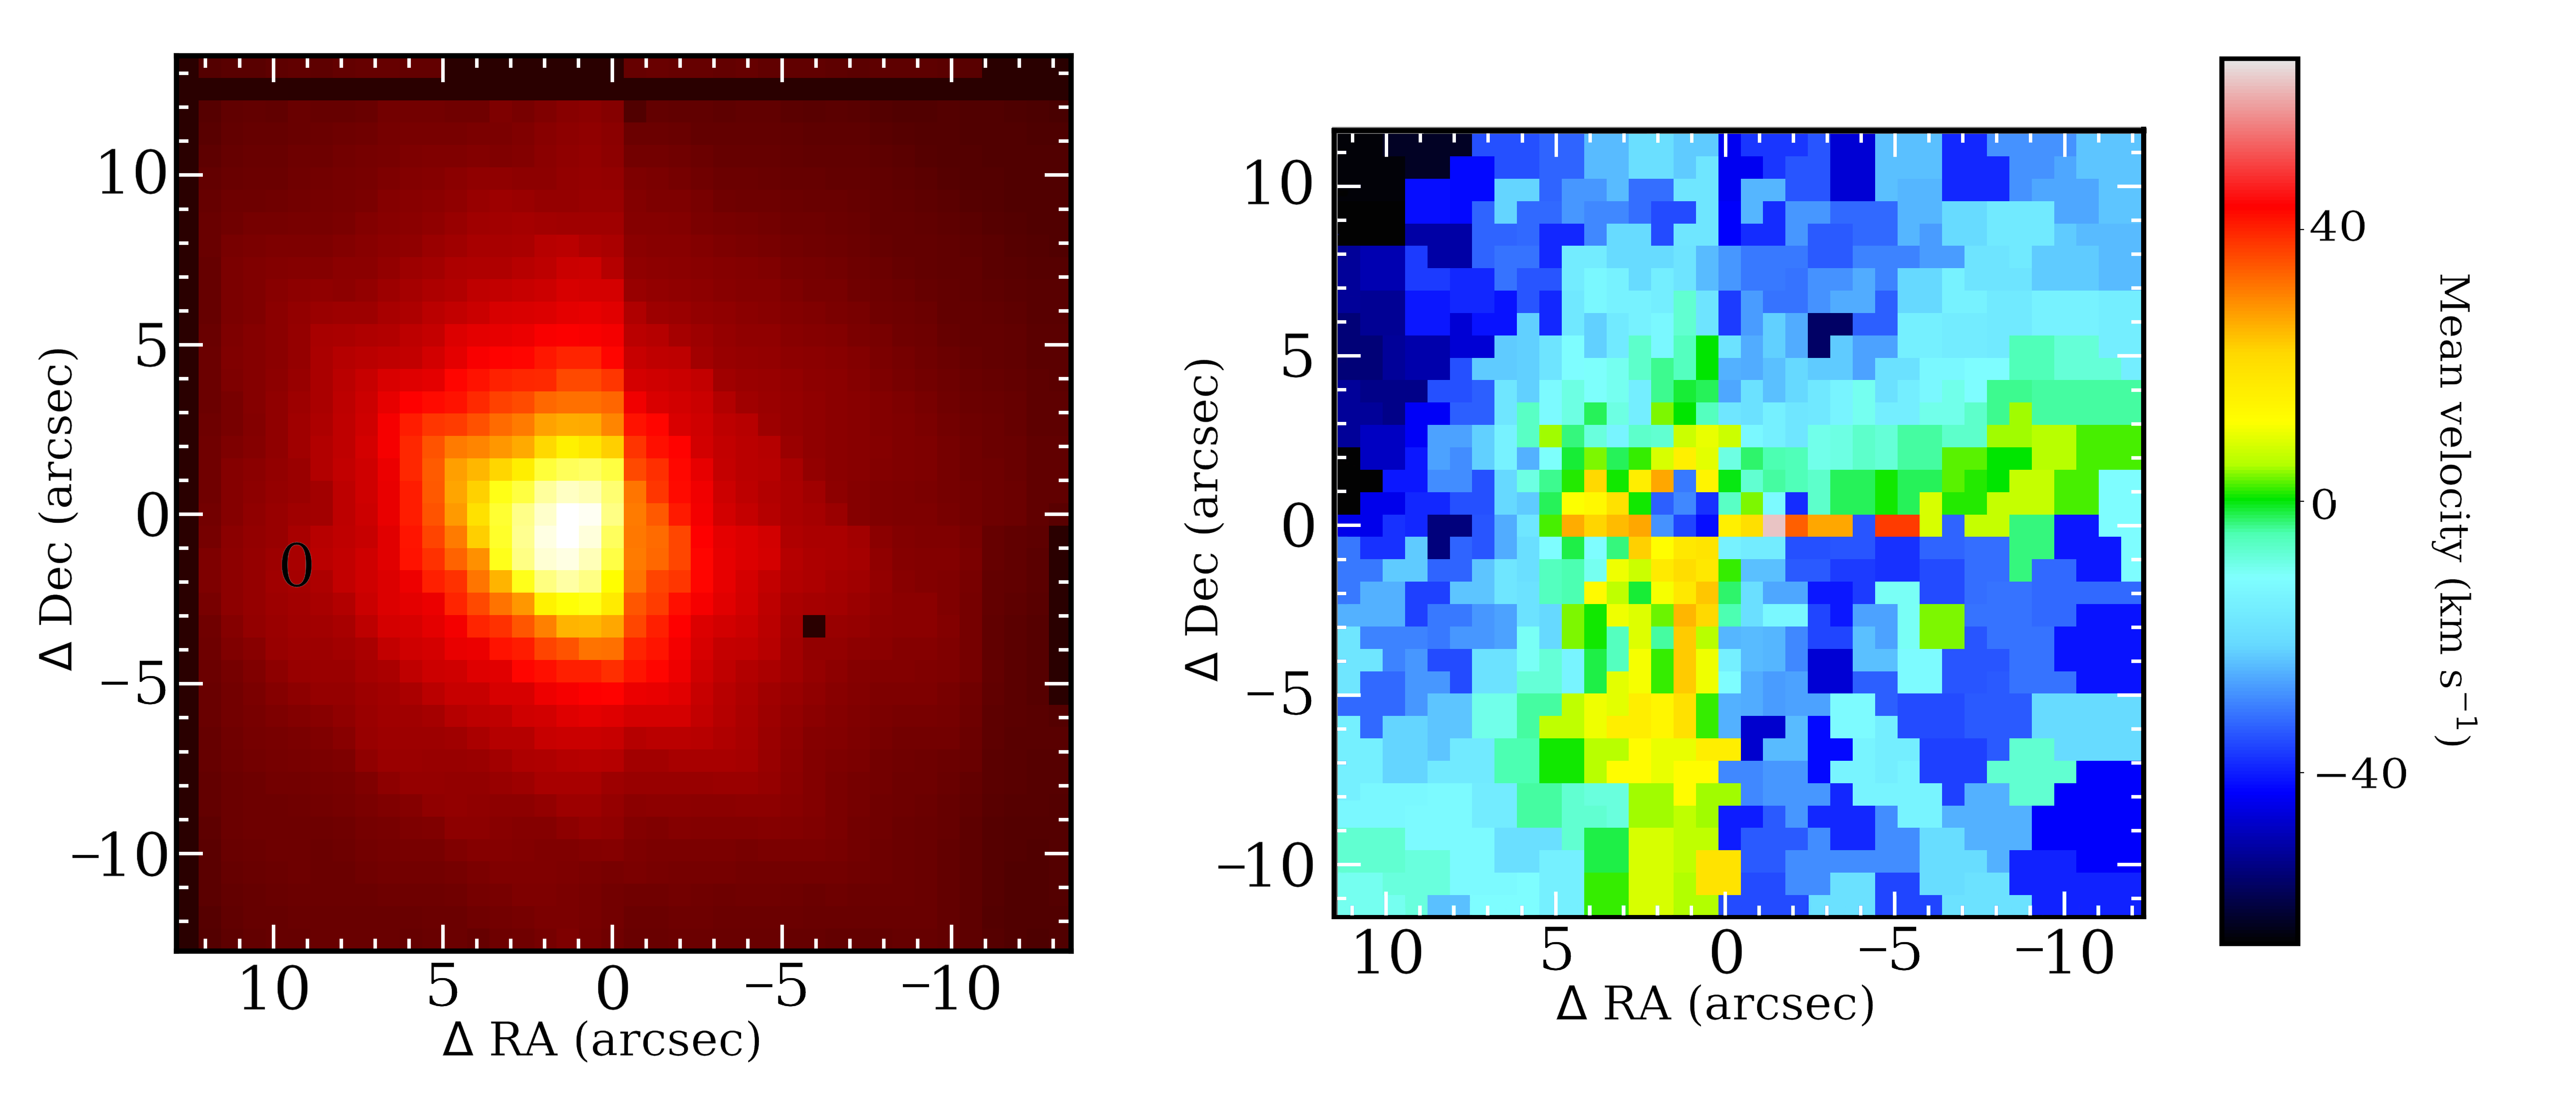
\includegraphics[width=.9\textwidth]{chapter2/P3D_NGC1399.png}
			\caption[\textsc{P3D}-reduced data problems]{Examples of problems with \textsc{P3D}-reduced data. Right panel: flux map (reconstructed image) of NGC 1399 Left panel: mean stellar velocity map of NGC 1399. Both maps show sharp offsets between the quadrants. The outer 2 spaxels on all sides of the velocity map were discarded.}
			\label{fig:P3D}
		\end{figure}


		The \textsc{p3d} wavelength-calibration step was not very successful either, as sharp offsets remain between the quadrants in the spectral direction. While this was still the case with \textsc{Py3D}-reduced data, the issue was much worse and more prevalent for \textsc{P3D}-reduced data. For example, the right panel of Fig.\,\ref{fig:P3D} shows the mean stellar velocity map of NGC 1399 extracted from \textsc{P3D}-reduced data. The wavelength calibration is so bad that rotation pattern of the galaxy is completely obfuscated.

		
\section{Multi-unit Spectroscopic Explorer (MUSE)}
	\label{sec:MUSE}

	\subsection{MUSE Instrument}
		The Multi-unit Spectroscopic Explorer (MUSE) is located on UT4 of ESO's VLT. It is comprised of 24 channels, each feeding an IFU (image slices) and spectrographs for a total contiguous field of view of $1\arcmin \times 1\arcmin$ at spatial sampling of $0\farcs2$. It has a spectral range of 4800-9300\,\AA\ with a spectral resolution of $\approx 2.3$\,\AA\ sampled at 1.25\,\AA\,pix$^{-1}$. MUSE is currently offered with and without adaptive optics (AO), and a narrow-field mode (with an order of magnitude improvement in spatial resolution and sampling) is planned for the future. 
		
	\subsection{MUSE Archival Observations}
		Four of the sample galaxies are in the MUSE archive: IC 1459, IC 1531, NGC 1316 and NGC 1399. NGC 1316 (observed as part of programme 094.B-0298A) and NGC 1399 (programme 094.B-0903A) where both observed as mosaics, while IC 1459 and IC 4296 (both also programme 094.B-0298A) where observed in single pointings. All were observed in service mode during ESO period 94, in the MUSE wide-field mode without adaptive optics . Every OB in both programmes followed the standard MUSE calibration plan.

	\subsection{MUSE Data Reducing}
		\label{subsec:MUSEreduction}
		
		Because the computing resources required to reduce raw MUSE data are very large, the data quality is high, and the pipelines products are known to be robust, we adopt for this project the pre-reduced (known as Phase 3) data products from ESO, so that the ESO data reduction pipeline\footnote{http://www.eso.org/sci/software/pipelines/muse/muse-pipe-recipes.html} is already applied. 

		The ESO pipeline contains all standard IFU data reduction steps: bias subtraction, flatfielding of detectors using continuum lamp exposures, flatfielding of fibres using twilight exposures, wavelength calibration, flux calibration using standard stars and sky subtraction (both programmes included dedicated sky exposures). Tiled observations, where present, are combined into a final mosaic.

		We found that the Phase 3 data products were indeed generally of a sufficient quality for our purposes, except that in both IC 1459 and IC 4296 the sky appears to have been over-subtracted. The ESO Phase 3 data release description for MUSE\footnote{https://www.eso.org/sci/observing/phase3/data_releases/IDP_MUSE_IFU_release_description_1.0.pdf} points out that the automatic data-reduction routine does not verify stable conditions (such as photometry and moon visibility) before applying the sky subtraction. Unstable conditions may well be the source of over subtraction which manifested itself as enormous apparent absorption features (often with negative fluxes) in the spectra. To remove this over-subtraction, we developed our own pseudo-sky subtraction routine. A median spectrum was taken from four $20 \times 20$\,spaxel regions, one in from each spatial corner of the ESO reduced cube. After checking that no stellar continuum could be fit to the medium sky spectrum (i.e.\ that very little light from the galaxy is contaminating the pseudo-sky regions), this median sky spectrum was subtracted from each spaxel in the cube. 

		This extra (pseudo-)sky subtraction was not possible for NGC 1316 and NGC 1399 due to mosaic nature of the observations, since this sky subtraction should be applied to each exposure of the mosaics independently (while the different exposures are already combined as part of the automated data reduction). It is also impossible to access data products from intermediate steps in the data-reduction process, such as immediately before the mosaic is produced. Fortunately, both NGC 1316 and NGC 1399 are not as badly affected by poor sky subtraction as IC 1459 and IC 4296, so they are left uncorrected. 

		Finally, we trimmed all the cubes to the central $30\arcsec \times 30\arcsec$ ($150 \times 150$\,spaxels) only, to (a) avoid the regions used for the pseudo-sky spectrum and (b) reduce the computing resources required for spatial binning (see Section \ref{sec:analysis}). In any case, the bins would be so large in the outer parts as to be effectively useless (see Fig\,\ref{fig:egSNR}).

		As for the VIMOS data, the variance spectra are propagated throughout the entire data-reduction pipeline, including our additional pseudo-sky subtraction step, and are squared-rooted at the end, to be used as noise inputs at the analysis stage. 

\section{Data Analysis}
	\label{sec:analysis}
	From this point on, the VIMOS and MUSE datasets are treated almost identically, the only difference (other than the different spectral ranges and resolutions) being that the MUSE datacubes are binned to a higher signal-to-noise ratio (S/N).

	For each galaxy (i.e.\ each combined cube), the data analysis process can summed up as follows, each step being detailed below:
	\begin{enumerate}
		\item Spatially bin the spectra using Voronoi binning.
		\item Identify the relevant stellar templates, by fitting the entire galaxy spectrum (obtained by summing all galaxy spectra) with all the templates from the Miles library, and hereafter using only the non-zero weight templates.
		\item Estimate the redshift and velocity dispersion of the entire galaxy spectrum with a Markov chain Monty Carlo (MCMC) routine. 
		\item Find the best-fit line-of-sight velocity distribution (LOSVD; as parametrised by the Gaussian parameters $v$, the mean velocity and $\sigma$, the velocity dispersion) of the stellar and ionized gas components in each bin, using a bootstrapping method to estimate the uncertainties on the measurements. 
		\item Remove the fitted emission lines and measure the absorption line strengths in each bin. 
		\item Identify the best-fit stellar population model in each bin using the measured absorption line strengths.
	\end{enumerate}


	\subsection{Spatial Binning}
		\label{subsec:Binning}
		Given that galaxies are brightest at their centres and fade away radially, and that the noise (assumed to be Poisson dominated) scales as the square root of the signal, the S/N of the galaxy spectra will also be highest at the galaxy centres, decreasing with increasing radius. In the outer regions of galaxies, the S/N becomes too low to extract meaningful information from the spectra. Because of this, we spatially bin the spectra to a fixed target S/N (increasing a bin's size until it reaches the required S/N). This is performed using the adaptive Voronoi binning routine\footnote{http://www-astro.physics.ox.ac.uk/~mxc/software/} of \citet{Cappellari2003}. For our purposes, we define the `signal' and `noise' of each spaxel as the median value of its spectrum and noise spectrum, respectively. We require a S/N of 30 for all VIMOS datacubes and 50 for the IC 1459 and IC 4296 MUSE datacubes. The NGC 1316 and NGC 1399 MUSE datacubes were binned to a S/N of 50 for the analysis of the stellar kinematics and 100 for the analysis of the emission line kinematics and stellar populations. These target S/N were chosen in order to be as low as possible, while still returning meaningful information (as assessed by eye). The NGC 1316 and NGC 1399 MUSE datacubes have different S/N thresholds due to the extra (pseudo-)sky subtraction applied to the IC 1459 and IC 4296 datacubes, that were successful at removing artefacts from the spectra (thus allowing us to retain a higher level of spatial information for these two galaxies). The remaining artefacts in NGC 1316 and NGC 1399 datacubes did not seem to affect the analysis of the stellar kinematics, but did affect the emission line fits, so we enforced a higher S/N threshold for the emission line analysis and where careful subtraction of the emission lines is important (i.e.\ in the analysis of the stellar populations). 

		Figure \ref{fig:egSNR} shows an example of the Voronoi bins. Concentric rings can clearly be seen around the centre of the galaxy, as bins with a S/N just below the target are increased in size by a single spaxel, resulting in a final S/N well over the target. Spaxels within the first ring are not binned and can have arbitrarily high S/N (dictated by the galaxy surface-brightness profile), while bins outside the central rings are composed of many spaxels and naturally have S/Ns clustered around the target value.

		\begin{figure}
			\centering
			\includegraphics[width=.6\textwidth]{chapter2/egSNR.png}
			\caption[Example signal-to-noise map]{Example signal-to-noise ratio (S/N) map, from the MUSE observations of IC 1459.}
			\label{fig:egSNR}
		\end{figure}

	\subsection{Stellar Kinematics}
		\label{subsec:StellarFit}
		Our analysis makes use of the penalized-fitting routine \textsc{pPXF}\footnote{http://www-astro.physics.ox.ac.uk/~mxc/software/} by \citet{Cappellari2004, Cappellari2016a}. This routine finds the best-fitting kinematics by minimizing the reduced chi-squared of a fitted spectrum built from combined empirical stellar templates, convolved with a Gaussian line-of-sight velocity distribution (LOSVD; here parametrised by the mean velocity, $v$, and velocity dispersion, $\sigma$, only). Gaussian templates can also be used to fit emission lines from the interstellar medium (ISM) as independent components (with their own LOSVD). \textsc{pPXF} requires an initial guess for the LOSVD for each component. We use the redshift of the galaxy and $200\,\mathrm{km\,s^{-1}}$ for the initial velocity and velocity dispersion estimates. Finally, Lagrange polynomials can be used to make additive or multiplicative corrections to the continuum level of the fit. A possible sky line at 5199\,\AA\ in the Earth's frame of reference is masked in all fits.

		In order to improve the speed of our analysis, we first collapse the datacube spatially to give a global spectra for the galaxy by summing across both spatial dimensions at each wavelength. Then the entire Miles stellar library \citep{Sanchez-Blazquez2006, Falcon-Barroso2011a} is used as templates for \textsc{pPXF} to fit. $600\,\mathrm{km\,s^{-1}}$ wide regions around possible emission lines (see Table \ref{tab:EmissionLine}) are masked and a fourth order Lagrange polynomial is used for an additive continuum correction. We use the redshift values from Simbad \citep{Wenger2000} for our initial velocity estimate. For our 14 datacubes (10 VIMOS and 4 MUSE), this step fits an average of 23 templates out of 985 with a non-zero weighting. Zero-weighted templates are discarded in future analysis of a given datacube. This drastically improves the runtime of \textsc{pPXF} without effecting the quality of the fit.

		% For this fit the redshift from Simbad is used to move the spectra to the rest frame such that an initial guess of the velocity within that frame is 0 km s$^{-1}$. We use a initial guess of the velocity dispersion of 200 km s$^{-1}$ since ETGs have dispersions of around this value and higher. 



		%Regions (600 km s$^-1$ wide) around possible emission lines were masked. Emission lines included were: [OII]3726 , [OII]3729, H$_\delta$, H$_\gamma$, H$_\beta$, [OIII]4959, [OIII]5007, [NI]5199, [NI]5202, [OI]6300, [OI]6364, [NII]6548, [NII]6583, H$_\alpha$, [SII]6716 and [SII]6731. A telluric line at 5199 \AA, seen in some of the VIMOS spectra, was also masked, though the exact location of this depended on the initial redshift 'guess' since the spectrum is moved to the rest frame of the galaxy. For this analysis, we also allowed an additive continuum correction using a fourth order Lagrange polynomial.

		Next we run a MCMC routine to find more optimum initial estimates for velocity and velocity dispersion. For each observation, the initial run is set up in the same way as the previous step (though only using the templates with non-zero weightings). After each run, the fitted velocity and velocity dispersion are used as the initial estimate for \textsc{pPXF}, thus iteratively improving the initial guess with each subsequent run. After the first three repetitions, the velocity was used to calculate the precise redshift of the galaxy: these are the redshift values quoted in \ref{tab:sample}. After this, small random perturbations to the iterative initial estimates are applied to ensure that the routine converges on a global minimum chi-squared, rather than a local one. 100 repetitions are run, with the mean velocities and velocity dispersions recorded and used as the initial estimates for all subsequent fits in that datacube. 

		Beyond this point, each bin is analyzed independently. Each one is processed through \textsc{pPXF} using only the Miles templates with non-zero weighting from above, using the redshift, additional velocity and dispersion estimates from the last step as the initial required estimate. Again regions around emission lines are masked, and a fourth order additive continuum correction is used. To allow accurate estimation of the propagation of uncertainties in the best-fitting values, a bootstrapping method with 1000 repetitions is used. In each iteration (after the first), random noise, distributed with a Gaussian profile and an amplitude comparable to the noise propagated through the data reduction pipeline, is added to the best-fitting spectrum from the first run. The standard distribution of the fitted parameters from each iteration is used as the quoted uncertainty.


	\subsection{Emission-line Kinematics}
		\label{subsec:EmissionFit}
		Fitting emission lines is achieved in a similar fashion to finding the stellar kinematics. However, in order to combat template mismatches, where emission lines are erroneously fitted to the edges of absorption features that are under represented bu the stellar templates, we follow the method set out in \citet{Sarzi2005}. This is a three step process.
		\begin{enumerate}
			\item The region around each emission line's rest frame wavelength is masked, and the stellar spectrum is fitted.
			\item The kinematics of the stellar spectrum is fixed to the kinematics found in step 1. The region around the [\ion{O}{iii}] doublet is then unmasked and fitted.  
			\item All emission lines are unmasked, but have their kinematics fixed to that found for [\ion{O}{iii}] in Step 2. The emission lines are therefore being fitted with their amplitudes as their only free parameter. 
		\end{enumerate}
		All steps are repeated with the MC method described above to propagate uncertainties and include a tenth order multiplicative Lagrange polynomial to account for continuum emission. 

		The residuals between the best-fitting spectra and the input spectra are smoothed and averaged using a weighted, moving average. This is then summed in quadrature with the noise spectrum to give a combined `residual noise' spectrum. For each fitted emission line, $i$, the amplitude (of the fitted line) to the median residual noise (in the region of the emission line) ratio $(A/N)_i$. is used as a detection threshold. As in \citet{Sarzi2005}, a fit for [\ion{O}{iii}] only is considered a detection if $(A/N)_{[\text{\ion{O}{iii}}]} \ge 4$. For all other lines, $i$, except [\ion{N}{i}], a detection is recorded if [\ion{O}{iii}] is detected in the same bin and $(A/N)_\mathrm{i} \ge 3$; while a detection of [\ion{N}{i}] requires a detection of both [\ion{O}{iii}] and H\,$\beta$ and $(A/N)_{[\text{\ion{N}{i}}]} \ge 4$. Emission lines included are given in Table \ref{tab:EmissionLine} along with their rest wavelengths and that of any doublet counterparts (for so-called forbidden lines). 

	 	\begin{table}
	 		\centering
	 	\begin{threeparttable}
	 		\caption{Emission lines included in \textsc{pPXF} fit.}
	 		\label{tab:EmissionLine}
	 		\begin{tabular}{l c c}
	 		\hline
	 		\hline
	 		Line name 		& Emission line & Doublet counterpart  \\
	 		 & rest-frame wavelength (\AA) & wavelength (\AA) \\
	 		\hline
	 		\bracket{\ion{O}{ii}} 	& 3726.03 & 3728.82 \\
	 		H\,$\delta$ 	& 4101.76 \\
	 		H\,$\gamma$ 	& 4340.47 \\
	 		H\,$\beta$ 		& 4861.33 \\
	 		\bracket{\ion{O}{iii}}	& 4958.92 & 5006.84 \\
	 		\bracket{\ion{N}{i}} 	& 5199.36 & 5201.86 \\
	 		\bracket{\ion{O}{i}} 	& 6300.30 & 6363.67 \\
	 		\bracket{\ion{N}{ii}} 	& 6548.03 & 6583.41 \\
	 		H\,$\alpha$ 	& 6562.30 \\
	 		\bracket{\ion{S}{ii}} 	& 6716.47 & 6730.85 \\
	 		\hline
	 		\hline
	 		\end{tabular}
	 	\end{threeparttable}
	 	\end{table}




	 \subsection{Stellar Populations}
	 	\label{subsec:PopFit}
	 	In order to investigate the stellar populations of our sample we assume that a given spectra (a global, spatially integrated spectrum or the spectrum from a given bin) is well approximated to a simple/single stellar population (SSP), i.e.\ that spectrum represents a system of stars all born at the same time, in the same environment. 

	 	There are two methods for finding the best-fitting SSP: full spectral fitting of synthetic spectra with different properties or compare the observed absorption line strengths to empirical or modeled line strengths. The former has the advantage of retaining more information, being able to fit fine structure in the spectrum and can easily find complex stellar populations. It does, however, rely on highly reliable synthetic spectra for each permutation of stellar population properties that is considered. Also, for massive ETGs, fine structures in spectra are lost because of the smoothing from the high velocity dispersions. 

	 	The latter has the advantage of only considering the parts of the spectrum that are highly sensitive to the stellar population. It can be more easily based on empirical observations of stars in the solar neighborhood and thus is less model dependent. Interpolation between well populated regions of the parameter space of the stellar population properties can be used to minimize the errors in sparse regions of the parameter space. We also found that full spectral fitting almost always returned models from an extreme corner of the parameter space of models. For these reasons we use the absorption line strength approach.

	 	\subsubsection{Absorption Line Strengths}
	 		\label{subsubsec:Absorption}
	 		Absorption line strengths are measured as an equivalent width of a given index. Each index consists of 3 bandpasses: one blue and one red continuum bandpass on either side of the central bandpass containing the absorption feature. A pseudo-continuum is defined as a straight line between two points at the centre of each continuum bandpass with heights of the median intensity of the given bandpass. The index, $I$, is measured as the equivalent width of the spectrum, $F_\mathrm{I}(\lambda)$, within the central bandpass (defined between wavelengths $\lambda_1$ and $\lambda_2$) with respect to this pseudo-continuum, $F_\mathrm{C}(\lambda)$, i.e for the so-called atomic indices, measured in \AA,
	 		\begin{align}
	 			I_\text{\AA} \equiv \, & \int^{\lambda_2}_{\lambda_1} \! \left(1 - \frac{F_\mathrm{I}(\lambda)}{F_\mathrm{C}(\lambda)}\right) \, \mathrm{d}\lambda \, , \\
	 		\intertext{while molecular indices, measured in magnitude units is}
	 			I_\text{mag} \equiv \, & -2.5 \log\left(\frac{1}{\lambda_2 - \lambda_1} \int^{\lambda_2}_{\lambda_1} \! \frac{F_\mathrm{I}(\lambda)}{F_\mathrm{C}(\lambda)} \, \mathrm{d}\lambda\right) \, .
	 		\end{align}
	 		The indices we use for this project, along the defining bandpasses are taken from \citet{Trager1998} and are given in Table \ref{tab:abIndex}.


		 	\begin{table}
				\centering
			\begin{threeparttable}
				\caption{Definitions of bandpasses for line indices.}
				\label{tab:abIndex}
				\begin{tabular}{l c c c}
					\hline
					\hline
					Index 	& Blue cont. 		& Index band 		& Red cont. \\
					\hline 
					G4300 	& 4266.375--4282.625 & 4281.375--4316.375 & 4318.875--4335.125 \\
					Fe4383 	& 4359.125--4370.375 & 4369.125--4420.375 & 4442.875--4455.375 \\
					Ca4455 	& 4445.875--4454.625 & 4452.125--4474.625 & 4477.125--4492.125 \\
					Fe4531 	& 4504.250--4514.250 & 4514.250--4559.250 & 4560.500--4579.250 \\
					H\,$\beta$ & 4827.875--4847.875 & 4847.875--4876.625 & 4876.625--4891.625 \\
					Fe5015 	& 4946.500--4977.750 & 4977.750--5054.000 & 5054.000--5065.250 \\
					Mg\,b 	& 5142.625--5161.375 & 5160.125--5192.625 & 5191.375--5206.375 \\
					Fe5270 	& 5233.150--5248.150 & 5245.650--5285.650 & 5285.650--5318.150 \\
					Fe5335 	& 5304.625--5315.875 & 5312.125--5352.125 & 5353.375--5363.375 \\
					Fe5406 	& 5376.250--5387.500 & 5387.500--5415.000 & 5415.000--5425.000 \\
					Fe5709 	& 5672.875--5696.625 & 5696.625--5720.375 & 5722.875--5736.625 \\
					Fe5782 	& 5765.375--5775.375 & 5776.625--5796.625 & 5797.875--5811.625 \\
					NaD 	& 5860.625--5875.625 & 5876.875--5909.375 & 5922.125--5948.125 \\
					TiO1 	& 5816.625--5849.125 & 5936.625--5994.125 & 6038.625--6103.625 \\
					TiO2 	& 6066.625--6141.625 & 6189.625--6272.125 & 6372.625--6415.125 \\
					\hline
					\hline
				\end{tabular}
				\begin{tablenotes}
				\footnotesize
				\item \textit{Notes:} Indices are from \citet{Trager1998}.
				\end{tablenotes}
			\end{threeparttable}
			\end{table}

			Much of the literature measures absorption line strengths under the Lick/Cassegrain image dissector scanner spectrograph system (hereafter Lick/IDS system; \citealt{Faber1985, Worthey1994}). This has several disadvantages. Firstly, the Lick/IDS system is based on non-flux calibrated spectra from the IDS spectrograph on the Shane telescope (Lick Observatory), which has a relatively low and wavelength-dependent spectral resolution. When using the Lick/IDS system with other instruments, it is thus necessary to calibrate the observations by performing empirical corrections to correct for the uncalibrated continuum of the Lick/IDS data. This requires observations of standard stars with the same instrumental set-up as the main observations. Since this was not requested as part of the VIMOS observing strategy, we are not able to do this (a later proposal was not possible either as VIMOS was substantially upgraded in the intervening time). Given the low spectral resolution and poor data quality on which the Lick/IDS system is based, we believe in any case that the community should be making a concerted effort to use alternative systems. We therefore choose to use an alternative: the line index system (LIS) of \citet{Vazdekis2010}. LIS is based on flux calibrated measurements as several resolutions (5.0, 8.4 and 14.0\,\AA). \citet{Vazdekis2010} also provide empirical cubic functions for transforming literature measurements from the Lick/IDS system to LIS\footnote{http://www.iac.es/proyecto/miles/pages/line-index-system-lis/transformations.php}.

			Because of the models we use for stellar population fitting (detailed in Section \ref{subsubsec:StellarPop}), we actually measure absorption indices at a resolution of 2.5\,\AA\ (FWHM). For the purposes of comparisons to the literature (see Section \ref{subsec:absorption}) we also measure the absorption indices at 8.4\,\AA\ resolution. 

			Since the aim is to find the best-fitting stellar population is it important that we first remove the effect of the ISM. This involves fitting for (as described in Section \ref{subsec:EmissionFit}) and subtracting detected emission lines. 

			We must also correct for the effect of velocity dispersion of the stellar populations which will spread absorption features such that some of the absorption is outside of the central bandpass. To do this, we first build a spectrum that is not convolved with the velocity dispersion. This is done by creating the best-fitting spectrum (as in the previous step), but not convolving it with the LOSVD. A given index, $i$, is measured for both this `unconvolved' spectrum, ($I^\text{unc}_i$) and the convolved best-fitting spectrum ($I^\text{conv}_i$). The ratio of the indices measured for these two spectra is used as a (multiplicative) correction factor for the index measured on the emission line-corrected observed spectra ($I^\text{obs}_i$), such that
			\begin{equation}
				I^\text{corr}_i \equiv \frac{I^\text{unc}_i}{I^\text{conv}_i} I^\text{obs}_i \, .
			\end{equation}


		\subsubsection{Fitting Stellar Population Models}
			\label{subsubsec:StellarPop}
			The final step of the data analysis pipeline is to find the best-fitting SSP models for a given spectrum. Sets of SSP models consist of a grid of models characterised by stellar properties such as age ($t$), metallicity ($[Fe/H]$) and alpha-element enhancement ($\alpha$-enhancement; $[\alpha/Fe]$). Here, we first give an overview of the process of generating synthetic stellar populations before detailing the specifics of the models used below. 

			Synthetic SSPs are created using the following components:
			\begin{itemize}
				\item the loci of a star of a given mass and metallicity, as they travel across the Hertzsprung--Russel Diagram (HRD) by aging. These are known as stellar evolutionary tracks and are generally empirical.
				\item the function, $\Phi(M)$, representing the number of stars formed, $N(M)$, for a given mass, $M$, respect to mass. I.e.\ $\Phi(M) \equiv \frac{\mathrm{d}N(M)}{\mathrm{d}M}$. This is the initial mass function (IMF).
				\item an empirical library of stellar spectra to be able to assign a a spectra to a position on the HRD. 
			\end{itemize}
			The desired output of expected line strengths for a 3 dimensional grid of varying age, metallicity and $\alpha$-enhancement can be computed in one of two ways: (i) producing full synthetic spectra from the evolution of stellar atmospheres or (ii) finding a `fitting function' for each index which analytically calibrates the line strengths measured from empirical libraries to physical stellar parameters. The former is dependent on a good understanding of the physics of stellar atmospheres and is known to suffer from incomplete line lists and continuum uncertainties \citep{Thomas2004}. This would have been the appropriate method for producing spectra for full-spectral fitting had we chosen that method for investigating stellar populations (see Section \ref{subsec:PopFit}). The latter, and more popular method, interpolates between well populated regions of the parameter space. This allows the computing of the uncertainties in the model predictions and decreases those uncertainties in sparse regions of the parameter space. 

			ETGs often have very different fractional abundances of various metals to the nearby stars that we are able to observe (all of which have near solar abundances). As such, the stellar libraries that are used to calibrate the models fall short of the required coverage of the parameter space. Most methods make some effort to extrapolate to non-solar abundances. In a similar way to the fitting functions described above, `index response functions' can be found. This calibrates the effect of varying abundances of individual elements. In this case, comparison must be made to completely theoretical spectra.

			We use the SSP models by \citet{Thomas2010} (referred to hereafter as the TMJ models) as they are based on flux calibrated spectra and therefore do not require calibration to the Lick/IDS system. These models assume a \citet{Salpeter1955} IMF ($\Phi(M) \propto M^{-2.35}$) and are based on the evolutionary population synthesis code by \citet{Maraston1998}. The models use stellar evolutionary tracks by \citet{Cassisi1997} for metallicities of $[Z/H] < -0.33$ and \citet{Girardi2000} for $[Z/H] \ge -0.33$; the MILES stellar spectral library by \citet{Sanchez-Blazquez2006a} and \citet{Falcon-Barroso2011a}; fitting functions by \citet{Johansson2010} and index response functions by \citet{Korn2005}. The MILES library gives the models a resolution of 2.5\,\AA\ (FWHM). This is below the resolution of the reduced VIMOS data (at 3\,\AA), but we in Fig.\,\ref{fig:res} we show that this effect is negligible. Comparing the absorption line strengths measured at 2.5\,\AA\ and 3\,\AA\ for the MUSE datasets shows the most effected index is Fe5782 with a mean difference of 1\% between the index measured at 3\,\AA\ and 2.5\,\AA. All other indices show a few tenths of a percent difference. 

			\begin{figure}
				\centering
				\includegraphics[width=.7\textwidth]{chapter2/compare_resolutions.png}
				\caption[Resolution effects on absorption line index strengths]{The effect of resolution of the measure absorption line strength. This shows that we can assume the effect of a lower spectral resolution in the VIMOS spectra, compared to the TMJ models will be negligible.}
				\label{fig:res}
			\end{figure}

			The response functions by \citet{Korn2005} extend the work of \citet{Tripicco1995} who investigated the response functions of the original 21 Lick indices when the individual element abundance fractions are varied for 5 Gyr old SSP at solar metallicities. The new functions include varying metallicities, as well as individual element fractions, and are calculated for all 25 Lick indices. The effect of age on these response function was tested by computing them for 1 Gyr models and comparing them to the 5 Gyr models by \citet{Tripicco1995}. They found a 1\% difference for two indices (G4300 and Fe4383) and a significantly lower result for all other indices, concluding that age does not significantly effect the response functions.

			Finally, the individual element abundances are combined to give the alpha element enhancement parameter, $\alpha/Fe$. This is done following \citet{Trager2000} who grouped the elements into three categories: 
			\begin{itemize}
				\item enhanced, containing C, N, O, Na, Mg, Si, Ca and Ti (i.e.\ $\alpha$ and light elements); 
				\item depressed, containing Cr and Fe (i.e.\ iron peak elements); and
				\item fixed (all other elements). 
			\end{itemize}
			The fixed group are held with solar abundances, while the enhanced and depressed groups are scaled up and down respectively by the same factor. 

			The TMJ models return index strengths for a 3 dimensional grid ($t$, $[Z/H]$ and $[\alpha/Fe]$) with $t$ = 0.1, 0.2, 0.4, 0.6, 0.8, 1,2, 3,4, 5, 6, 7, 8, 9, 10, 11, 12, 13, 14, 15 Gyr; $[Z/H]$ = -2.25, -1.35, -0.33, 0.0, 0.35, 0.67 $\mathrm{[Z/H]_\odot}$; and $[\alpha/Fe]$ = -0.3, 0.0, 0.3, 0.5 $\mathrm{[\alpha/Fe]_\odot}$.

			\citet{Thomas2010} showed that the TMJ models produce a good fit to globular cluster measurements of \citet{Puzia2002} and \citet{Schiavon2005} and the galaxy measurements by the SAURON group by \citet{Kuntschner2010}. \citet{Conroy2010} suggests that the stellar evolutionary tracks by \citet{Girardi2000} used for the high metallicity models do not fit the globular clusters well, however \citet{Thomas2010} point out that this can be explained by an anomaly in the Balmer lines which is not seen in the analysis of the SAURON data. \citet{Thomas2010} therefore suggest, that this is an issue with the globular cluster observations themselves. 

			Following the method of \citet{McDermid2006} we first linearly interpolate the TMJ models to a 3-dimensional grid with sides of length 40 in age, metallicity and $\alpha$-enhancement. Metallicity and $\alpha$-enhancement directions are evenly spaced, while the age direction is logarithmically spaced. We then use \textsc{emcee}, a \textsc{python} package for MCMC fitting, to find the most-likely SSP model by comparing the absorption line strengths (measured with the method described in Section \ref{subsubsec:Absorption}) to the absorption line strengths of the SSP models. We take the standard deviation of the positions of the walkers in the MCMC code as the uncertainties.

			The following chapters will use results from these pipelines to compare our radio galaxy sample, the Southern Sample to radio-quiet ETGs.
